\section{Application Scenarios}
\label{sec:pswareImpl}
In previous sections, we have introduced PSWare and how it can be customized to meet different application requirements. In this section, we demonstrate how PSWare can help in developing practical WNS applications through three application case studies: the indoor monitoring, the car park and the intelligent transportation system.

The key features of the three applications are as follows:
\begin{itemize}
\item Energy efficiency in an indoor monitoring system is crucial because the network needs to operate for a long period of time and it is not necessary to gather all the raw data.
\item Reliability is important in a car park system because the management system needs to know the time when each car enters and leaves the car park so as to calculate the fee.
\item Event detection and delivery mechanism may be tailor-made for an ITS system.
\end{itemize}

\subsection{Application Overview}
An indoor monitoring system can have many different purposes including air-conditioning, fire alarm and office space light adjustment. Such system is a good application for using composite events because of the following characteristics:
\begin{itemize}
\item There may be a large amount of raw data since the data may be gathered from a lot of sources.
\item The users may not be interested in all the raw data. Instead, they may be more interested in change of the data. This is because the events such as fire or temperature change will usually trigger the change of the sensory data. 
\item Primitive event detection may not be sufficient. For instance, a fire alarm may be characterized by a combination of different types of events such as temperature and light.
\end{itemize}

To have a practical application scenario, we deployed our sensor nodes around the Internet and Mobile Computing Laboratory of the Hong Kong Polytechnic University. The deployment plan is shown in Figure \ref{fig:indoorDeployment}.

\begin{figure}
\centering
\figurecurrentwidth{indoorDeployment}
\caption{Deployment of the senosr nodes for indoor monitoring}
\label{fig:indoorDeployment}
\end{figure}

We use this deployment for two applications: fire detection and temperature control. Since it is infeasible to transmit all the raw data to the sink, some nodes in the network will have be used as local decision maker and detect the composite event. As a result, developing the application will involve the following steps:
\begin{enumerate}
\item Deploy the network and select the appropriate sensor nodes as event detectors. We borrow the idea from TED \cite{lai:ted} and call these event detectors event fusion points. In our deployment, we select the nodes 14, 16 and 0 as fusion points.
\item Subscribe the desired events through PSWare.
\item Detect the composite events with PSWare.
\item Automatically let the nodes switch between different event fusion points to achieve high efficiency.
\end{enumerate}

\subsection{Overall Architecture}
Based on our requirement analysis, we have the system architecture shown in Figure \ref{fig:indoor-architecture}. On the bottom layer, we have PSWare as well as a module for selecting event fusion points. During the event detection process, the fusion point selection will be executed in parallel and the sensor nodes will switch between fusion points to minimize the detection cost. The two modules interact with each other mainly through two interfaces: when an event is matched, the fusion selection module will be called to update the some tables so that when the event is detected again later, the module can be called again to select the better node for forwarding the event.

\begin{figure}
\centering
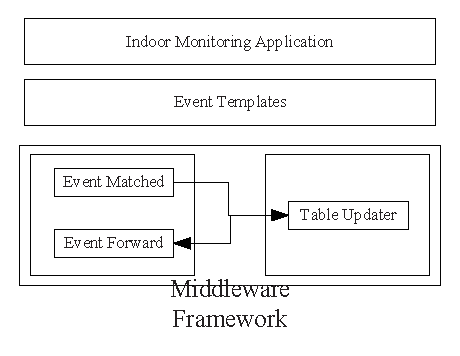
\includegraphics[width=.8\textwidth]{indoor-architecture}
\caption{Architecture of indoor application based on PSWare}
\label{fig:indoor-architecture}
\end{figure}

\subsection{Data Structures}
We used TED for fusion point selection, in this section, we will show what kind of data are maintained by individual sensor nodes so that they will later be used for efficient event detection. We have a set of nodes \(V'\subseteq V\) selected as event fusion points. Each individual sensor nodes will maintain the following table \(table_r\) for all \(v'_n\in V'\)
\begin{itemize}
\item Fusion point ID (\(fid_n\)): the node ID of the fusion point:
\item	Hop count (\(hop_n\)): the number of hops to reach the fusion point
\item	Parent (\(parent_n\)): the next hop to that fusion point\\
\end{itemize}
Each sensor node will also maintain an event table \(table_e\) containing the information for each event type \(e_n\in E\) which includes the following fields:
\begin{itemize}
\item Event type ID (\(e_n\)): the ID which is assigned to each event type
\item Fusion point for the event (\(fusion_n\)): the fusion point at which the event is mostly likely to be detected at the lowest cost.
\item Fusion cost (\(cost_n\)): the fusion cost for event type \(e_n\)\\
\end{itemize}
In addition to the above tables, each fusion point \(v'\in V'\) will maintain another table \(table_m\) for the purpose of matching events. \(table_m\) contains the following fields:
\begin{itemize}
\item Event type ID (\(e_n\)): the ID of the event type
\item Event instance ID (\(i\)): the \(i\)th event instance of event type \(e_n\) (we use \(e_n^i\) to denote such an instance of event)
\item Source node (\(v_n^i\)): the node which forwarded \(e_n^i\) to the fusion point
\item Event timestamp (\(t_n^i\)): the timestamp when the event \(e_n^i\) is detected
\item Detection cost (\(cost_n^i\)): the cost for detecting event \(e_n^i\)
\end{itemize}

\subsection{Table Construction}
Each node \(v_n\) periodically broadcasts messages \(msg_r\) which is its \(table_r\). If the node itself is a fusion point, then it will add itself in \(table_r\) and broadcast the message. The procedure is shown in Procedure \ref{algo:table_r}.

\begin{algorithm}
\begin{algorithmic}
\REQUIRE \(v_n\rightarrow msg_r\)
	\FOR {each entry \(t'\) in \(msg_r\)}
		\IF {\NOT exists \(t'\rightarrow fid_n\) in \(table_r\)}
			\STATE \(addTo(table_r, t')\)
		\ENDIF
		\FOR {each entry \(t\) in \(table_r\)}
			\IF {\(t\rightarrow fid_n = t'\rightarrow f_n\)}
				\IF {\(t'\rightarrow hop_n < t\rightarrow hop_n\)}
					\STATE \(t\rightarrow hop_n \gets t\rightarrow hop_n+1\)
					\STATE \(t\rightarrow parent_n \gets v_n\)
				\ENDIF
			\ENDIF
		\ENDFOR
	\ENDFOR
	\IF {self is fusion point \AND \NOT exists \(self\rightarrow id\) in \(table_r\)}
		\STATE \(addTo(table_r, (self\rightarrow id, 0, self\rightarrow id))\)
	\ENDIF
	\STATE \(msg_r \gets table_r\)
	\STATE \(periodically\_broadcast(msg_r)\)
\end{algorithmic}
\caption{\(table_r\) construction}
\label{algo:table_r}
\end{algorithm}

In addition to \(msg_r\), each \(v'_k\in V'\) will periodically advertise its \(table_m\) by broadcasting \(msg_m\) so that other sensor nodes can construct their \(table_e\) with Procedure \ref{algo:table_e}.

\begin{algorithm}
\begin{algorithmic}
\REQUIRE \(v'_k\rightarrow msg_m\)
	\FOR {each entry \(t'\) in \(msg_m\)}
		\IF {\NOT exists \(t'\rightarrow e_n\) in \(table_e\)}
			\STATE \(addTo(table_e, (t'\rightarrow e_n, 1, v'_k, t'\rightarrow cost_n^i+table_r\rightarrow hop_k))\)
		\ENDIF
		\FOR {each entry \(t\) in \(table_e\)}
			\IF {\(t\rightarrow e_n = t'\rightarrow e_n\)}
				\IF {\(t'\rightarrow cost_n^i+table_r\rightarrow hop_k < t\rightarrow cost_n\)}
					\STATE \(t\rightarrow cost_n \gets t'\rightarrow cost_n^i+table_r\rightarrow hop_k\)
					\STATE \(t\rightarrow fusion_n \gets v'_k\)
				\ENDIF
			\ENDIF
		\ENDFOR
	\ENDFOR
	\IF {self is fusion point}
		\STATE \(msg_m \gets table_m\)
		\STATE \(periodically\_broadcast(msg_m)\)
	\ENDIF
\end{algorithmic}
\caption{\(table_e\) construction}
\label{algo:table_e}
\end{algorithm}

The construction of \(table_m\) will take place when the event instance \(e_n^i\) is detected and forwarded to a fusion point \(v'_n\). We will discuss how forwarding could be done in the next subsection.
\subsection{Event Matching and Forwarding}
When an event \(e_n^i\) is detected at node \(v_k\), node will use \(table_r\) and \(table_e\) to decide how to forward the detected event to the fusion points so that higher level events can be detected. The pseudo code is shown in Procedure \ref{algo:eventforwarding}.

\begin{algorithm}
\begin{algorithmic}
\REQUIRE detected event \(e_n^i\)
	\IF {\(table_e\rightarrow fusion_n=null\)}
		\STATE \(event\_forward(e_n^i)\)
	\ELSE
		\STATE \(send(e_n^i, table_e\rightarrow fusion_n)\)
	\ENDIF
\end{algorithmic}
\caption{Event forwarding}
\label{algo:eventforwarding}
\end{algorithm}

In case the fusion point for event type \(e_n\) has not been decided, the node will forward the event to some of its closet fusion points using the \(event\_forward\) function according to TED. Upon the reception of \(e_n^i\) from \(v_k\), the fusion point will first update its own \(table_m\). Then it will check if there is any composite event \(e_{comp}\) which uses \(e_n\) and another event \(e_j\) as its sub-event (\(e_{comp}=comp(e_n, e_j)\)). The pseudo code of event matching is shown in Procedure \ref{algo:eventmatching}.

\begin{algorithm}
\begin{algorithmic}
\REQUIRE \(e_n^i\) detected by \(v_k\) with cost: \(cost_n^i\)
	\STATE \(addTo(table_m, (e_n, e_n^i, v_k, now(), cost_n^i))\)
	\FOR {each \(e_j\) in \(E\)}
		\IF {\(\exists r\in R\) \AND \(r=e_{comp}=comp(e_n, e_j)\)}
			\FOR {each \(e_j^k\) in \(table_m\)}
				\IF {\(comp(e_n^i, e_j^k)=true\)}
					\STATE \(addTo(table_m, (e_{comp}, e_{comp}^i, self, now(), cost_n^i+cost_j^k))\)
					\STATE \(detected(e_{comp})\)
				\ENDIF
			\ENDFOR
		\ENDIF
	\ENDFOR
	\STATE \(event\_forward(e_n^i)\)
\end{algorithmic}
\caption{Event matching}
\label{algo:eventmatching}
\end{algorithm}

Note that if \(e_{comp}\) has been successfully detected, the procedure will run function \(detected\) which, in turn, will execute Procedure \ref{algo:eventforwarding}. The procedure will also use \(event\_forward\) in the end to forward the detected event to other fusion node so that better fusion point may be found.

\subsection{Event Subscription}
To monitor the temperature change of the entire floor and adjust the air-conditioner accordingly, we need to define a composite event that comprises of the sub-events for individual room. For example, the air conditioner can be adjusted if several adjacent rooms' temperature rises too fast. The primitive and composite event definitions for this purpose are shown in Listing \ref{prog:indoorEvents}.

\begin{lstlisting}[caption=Event definition for temperature monitoring, label=prog:indoorEvents]
Event SingleTemp {
	int id=System.id;
	int temperature=System.temperature;
} where {
	temperature>THRESHOLD
}
Event CompositeTemp {
} on {
	SingleTemp e1, e2, e3;
} where {
	e1.id==1 &&
	e2.id==2 &&
	abs(e1.time - e2.time)<TIME_INTERVAL
}
\end{lstlisting}

The primitive event simply tests if the temperature passes certain threshold while the composite event is the conjunction of several primitive events. We deployed the some Micaz nodes in different rooms in our building as shown in Figure \ref{fig:indoorDeployment}.

For fire alarm, the composite event definition is based on both light and temperature readings. The event definition is shown in Listing \ref{prog:indoorFire}.
\begin{lstlisting}[caption=Event definition for fire alarm, label=prog:indoorFire]
Event Temperature {
	int id=System.id;
	int temperature=System.temperature;
} where {
	temperature>THRESHOLD_TEMP
}
Event Light {
	int id=System.id;
	int light=System.light;
} where {
	light>THRESHOLD_LIGHT
}
Event Fire {
} on {
	Temperature temp;
	Light light;
} where {
	e1.id==light.id
}
\end{lstlisting}